%
% File acl2019.tex
%
%% Based on the style files for ACL 2018, NAACL 2018/19, which were
%% Based on the style files for ACL-2015, with some improvements
%%  taken from the NAACL-2016 style
%% Based on the style files for ACL-2014, which were, in turn,
%% based on ACL-2013, ACL-2012, ACL-2011, ACL-2010, ACL-IJCNLP-2009,
%% EACL-2009, IJCNLP-2008...
%% Based on the style files for EACL 2006 by 
%%e.agirre@ehu.es or Sergi.Balari@uab.es
%% and that of ACL 08 by Joakim Nivre and Noah Smith

\documentclass[11pt,a4paper]{article}
\usepackage[hyperref]{acl2019}
\usepackage{times}
\usepackage{latexsym}
\usepackage{amsmath}
\usepackage{graphicx}
\usepackage{caption}
\usepackage{subcaption}
\DeclareMathOperator*{\argmax}{arg\,max}
\DeclareMathOperator*{\argmin}{arg\,min}

\usepackage{url}

\aclfinalcopy % Uncomment this line for the final submission
%\def\aclpaperid{***} %  Enter the acl Paper ID here

%\setlength\titlebox{5cm}
% You can expand the titlebox if you need extra space
% to show all the authors. Please do not make the titlebox
% smaller than 5cm (the original size); we will check this
% in the camera-ready version and ask you to change it back.
\newcommand\BibTeX{B\textsc{ib}\TeX}

\title{Concept Tagging for the Movie Domain}

\author{Giovanni De Toni (197814) \\
  University of Trento \\ Via Sommarive, 9, 38123 Povo,Trento TN\\
  \texttt{giovanni.detoni@studenti.unitn.it}}

\date{}

\begin{document}
\maketitle

\begin{abstract}
This work focuses on the well-known task of concept tagging phrase elements.
This present a relatively important challenge in the NLP field since it is
the starting point for more complex application. Weighted Finite State Transducer
and statistical method were used and an analysis of their performances is also provided.
\end{abstract}

\section{Introduction}
One of the first step of some NLP task is to analyze a given phrase to understand its underlying concept. For instance, imagine we are using a vocal application to order something to eat (e.g., "I would like a tortel di patate delivered at Piazza Trento 1, please"). In order for a machine to understand correctly what we want, firstly it needs to convert our utterances to a word representation, secondly it needs to assign concept to each of the word it heard (e.g., "tortel di patate" equals to requested food and "Piazza Trento 1" equals to the delivery address).
This basic operation is of utmost importance for all the application which can be built upon this. For instance, the quality of you food assistant is dependent on the quality of this concept tagger. Imagine what could happen if the machine were to swap the delivery address with the requested food!).  
The scope of this project is to provide a simple concept-tagger by developing a WSTF (Weighted Finite State Transducer) applied to the movie domain.
The report is detailed as follow: in the first section we define more formally the problem statement, then we proceed with an analysis of the given dataset and with the description of the models employed. Ultimately, we discuss the obtained results while underlying their stengths and limitations. 

\section{Problem Statement}
Given a sequence of tokens $<t_1, \ldots, t_n>$ and given a pool of concepts $<c_1, \ldots, c_m>$, we want to find the most likely assignment $<t_i, c_i>$ such that it maximizes the following probability:
\begin{equation}
c_1, \ldots, c_n = \argmax_{c_1, \ldots, c_n} P (c_1, \ldots, c_n | t_1, \ldots, t_n)
\label{frm:argmax}
\end{equation}
Thanks to the Markov assumption (the probability of the $i$-th concept depends only on the $(i-1)$-th concept and the probability of the $i$-th token depends only on the $i$-th concept), we can simplify the previous formula. Moreover, we can also compute its component by MLE (Maximum Likelihood Estimation):
\begin{equation}
c_1, \ldots, c_n = \argmax_{c_1, \ldots, c_n} P(t_i|c_i)P(c_i| c_{i-1})
\label{frm:argmax-markov-assumption}
\end{equation}
In the previous formula, $P(t_i|c_i) = \frac{C(c_i, t_i)}{C(c_i)}$ and $P(c_i|c_{i-1}) = \frac{C(c_{i-1}, c_i)}{C(c_i)}$ (where $C(x)$ counts the occurrences of $x$ inside the given dataset). 

\begin{table*}[b!]
    \begin{subtable}{.5\linewidth}
		\centering
\begin{tabular}{|l|l|}
\hline
\multicolumn{2}{|l|}{\textbf{NL2SparQL4NLU.trai.conll.txt}} \\ \hline
\textit{\# of lines}									& 24791 \\ \hline
\textit{\# of sentences}                             & 3338 \\ \hline
\textit{\# of unique tokens}                         & 1728 \\ \hline
\textit{\# of unique concepts (without the prefix)}  & 24   \\ \hline
\end{tabular}
\caption{Description of the content of the train dataset.}
\end{subtable}%	
\begin{subtable}{.5\linewidth}
\centering
\begin{tabular}{|l|l|}
\hline
\multicolumn{2}{|l|}{\textbf{NL2SparQL4NLU.test.conll.txt}} \\ \hline
\textit{\# of lines}									& 8201 \\ \hline
\textit{\# of sentences}                             & 1084 \\ \hline
\textit{\# of unique tokens}                         & 1039 \\ \hline
\textit{\# of unique concepts (without the prefix)}  & 23   \\ \hline
\end{tabular}
\caption{Description of the content of the test dataset.}
\label{tab:test-dataset-description}
\end{subtable}
\end{table*} 

\section{Data Analysis}

The dataset used is called NL2SparQL4NLU. This work used only the "*.conll.txt" files (more specifically, one for training the language model and one for testing it). Each file is written using the token-per-line CONLL format with tokens and NLU concept tags. An analysis of the content of the two files follows:

The distribution of the tokens was analyzed. It was found to behave accordingly to the
Zipf's Law, however, for brevity, it was not reported here since it was not showing 
anything interesting. The OOV rate for the tokens is around $23.68\%$. 
The distribution of the various concepts was also analyzed (both for the training
and the test datasets). The distribution of the various concepts is shown in Figure \ref{fig:concept-distribution}. It is possible to see how the \textit{movie.name} concept is one of the most common (followed by \textit{actor.name} and \textit{person.name}). However, it can also be noted that the ''\textit{O}" concept represent the $70\%$ of the dataset, which represent an issue for the following tagging procedure.

Both train and test set contains concepts which are not present in the other dataset (and viceversa). The train dataset contains \textit{person.nationality} (2 occurrences) and \textit{movie.description} (2 occurrences) which are not present in the test set. The test dataset contains the concept \textit{movie.type} which is missing from the train dataset (4 occurrences). These again could cause mistagging issues and therefore lower the final performance.
As a final note, there are also
some tokens which are the results of mispelling (e.g., "dispaly", "Scorcese") which therefore could lead to mistagging.


\section{Models}

In this work we devised four separated language models. 
The first language model was developed by using directly 
the dataset provided (without any other addition). It 
implements directly Formula \ref{frm:argmax-markov-
assumption}. The second model implements a solution 
provided by Gobbi et al. [add citation]. As the data 
analysis showed us, the majority of the dataset concepts 
are "\textit{O}" which are not informative enough. Gobbi 
et al. proposes to substitute each occurrences of the 
"\textit{O}" concept with the corresponding lemmatized 
token such to increase the final performances. 
The third and fourth models add to their pipelines an 
entity recognition tool which converts certain token(s) 
to an entity definition. This entity definition replace 
the previous token. This improvement was performed such to reduce the variability inside the dataset. Some tokens infact refer to the same entity, while they may have different values (e.g., \textit{nick fury} and \textit{robin} are both character names, even if they have different tokens). See Figure \ref{fig:entity-recognition} for an example of entity recognition.

\begin{figure}[h!]
\centering
	\includegraphics[width=1\linewidth]{img/entity}
	\caption{Example of entity recognition. For instance, the "\textit{ed harris}" tokens were recognized as a PERSON while "\textit{thirteen}" was recognized as number.}
	\label{fig:entity-recognition}
\end{figure}

Generally, the entire pipeline was composed by three main components:
\begin{itemize}
\item First
\item Secon
\item Third
\end{itemize}

\section{Experiments}

Several experiments were run to assess the quality of 
the concept taggers. As a metric, we tried to find the solution which maximize the \textit{F1-score} over the test set. For each provided solution, we perfomed an extensive hyperparameter search by trying several smoothing techniques and ngram sizes. Each solution was evaluated by using k-fold cross-validation and the best result was then recorded. Firstly, we evaluated the Language Model based directly on the given dataset without any further improvements. The best combination was then used as a baseline. Secondly, we computed a second improved baseline performance by using the solution provided by Gobbi et al. [add citation]. Ultimately, we evaluated the two SpaCy model variants (dataset with entity recognition and dataset with entity recognition plus "\textit{O}" tags replaced. The results are summarized in Table X.

The code employed for the project is publicy available on Github [add link]. The script were written using Python 3.6 and bash. OpenFST [add citation] and OpenNGRAM [add citation] libraries were used to build the WFST and the language model. SpaCy [add citation] library was used to perform entity recognition.
The experiments were run on a 8th-core Intel i7 CPU with 16GB of RAM. 

\begin{figure*}[h!]
	\begin{subfigure}[b]{0.5\linewidth}
		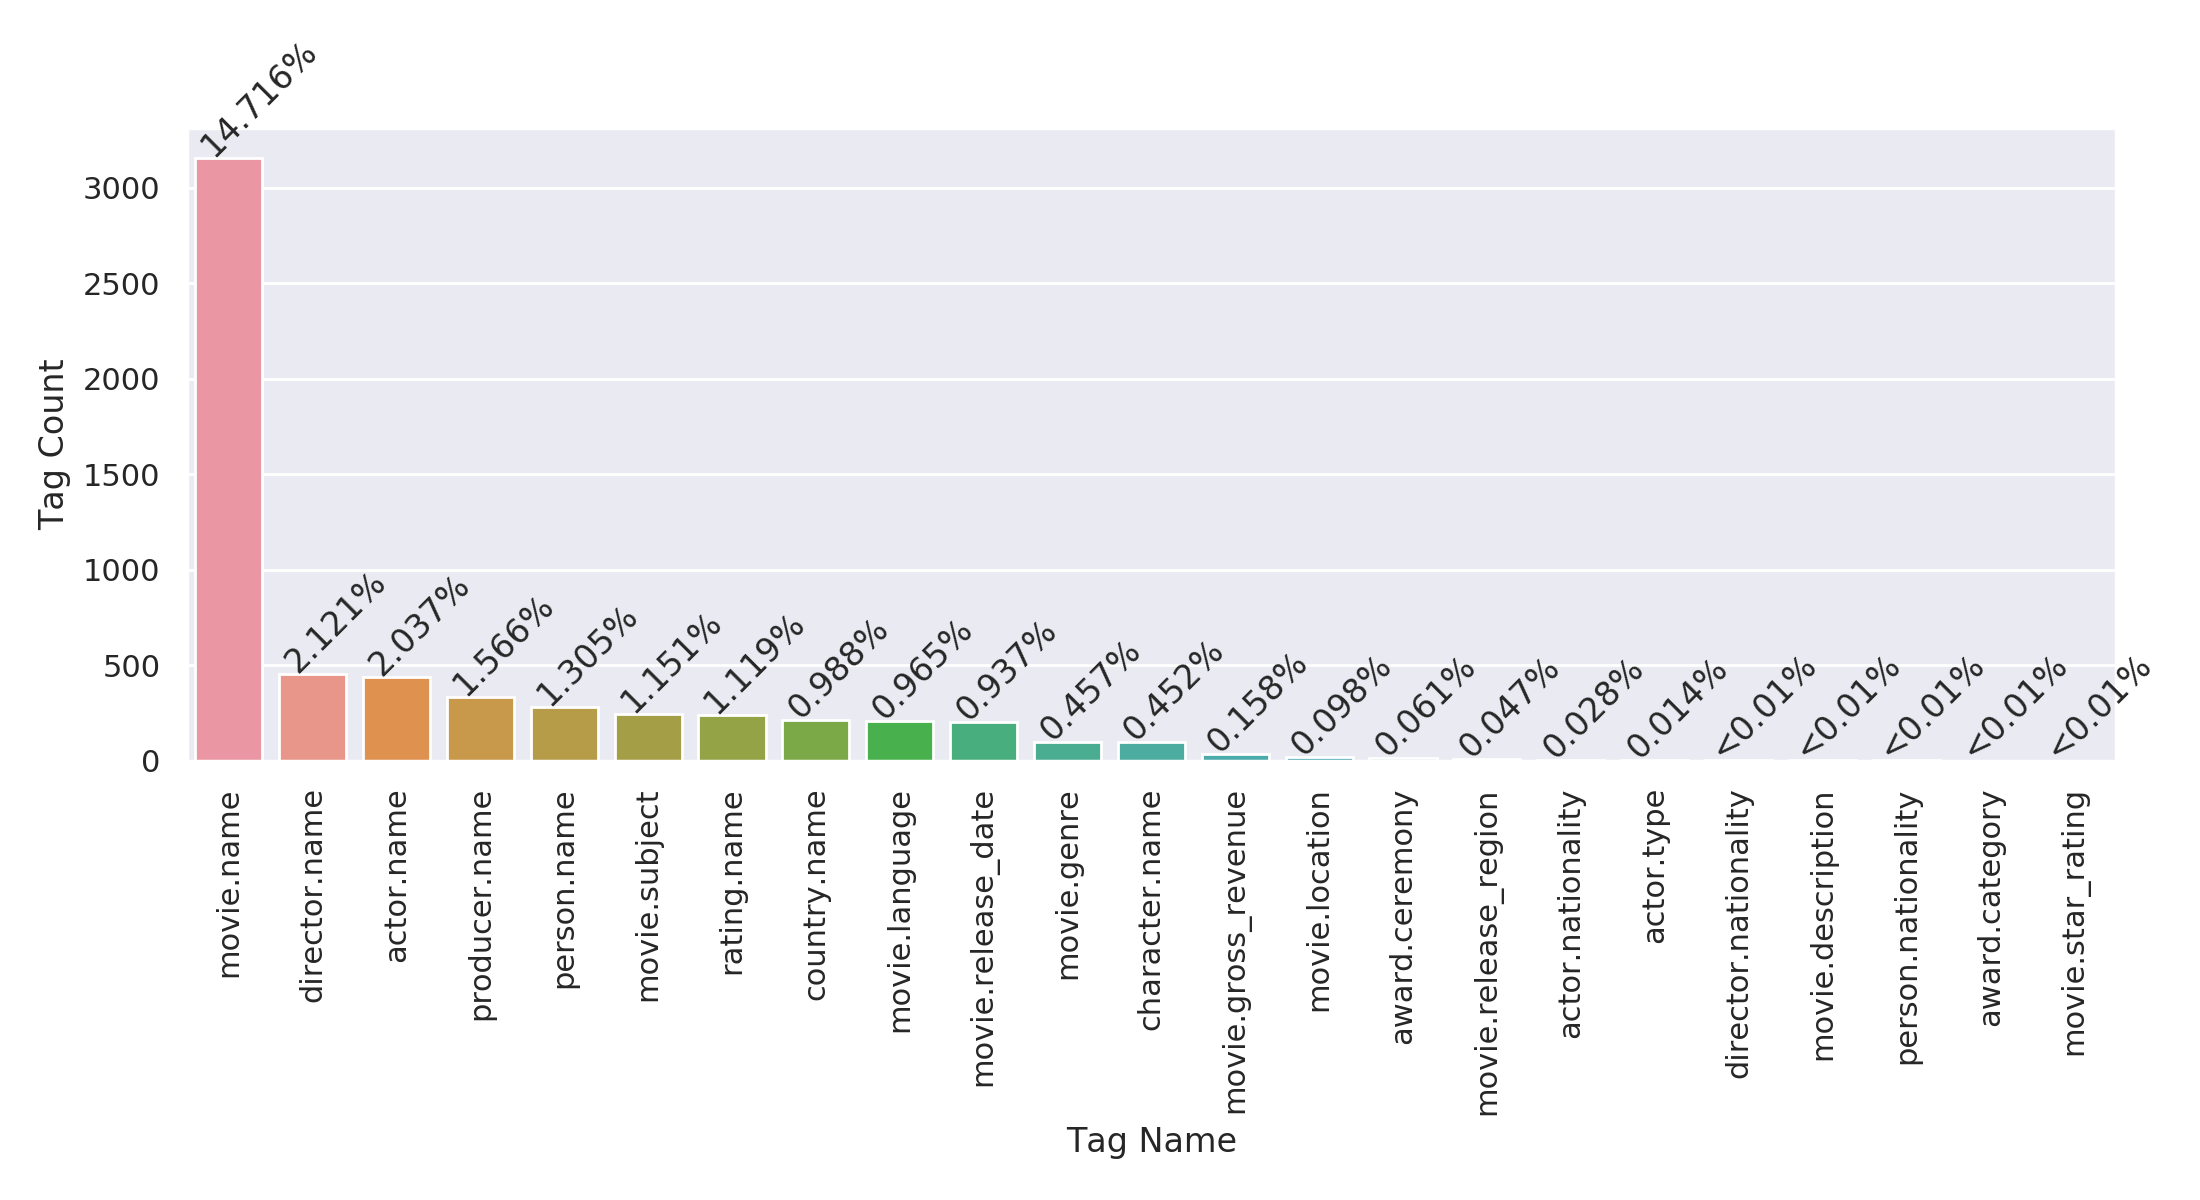
\includegraphics[width=\linewidth]{img/train-concepts-distribution}
		\caption{Train dataset.}
	\end{subfigure}
	\begin{subfigure}[b]{0.5\linewidth}
	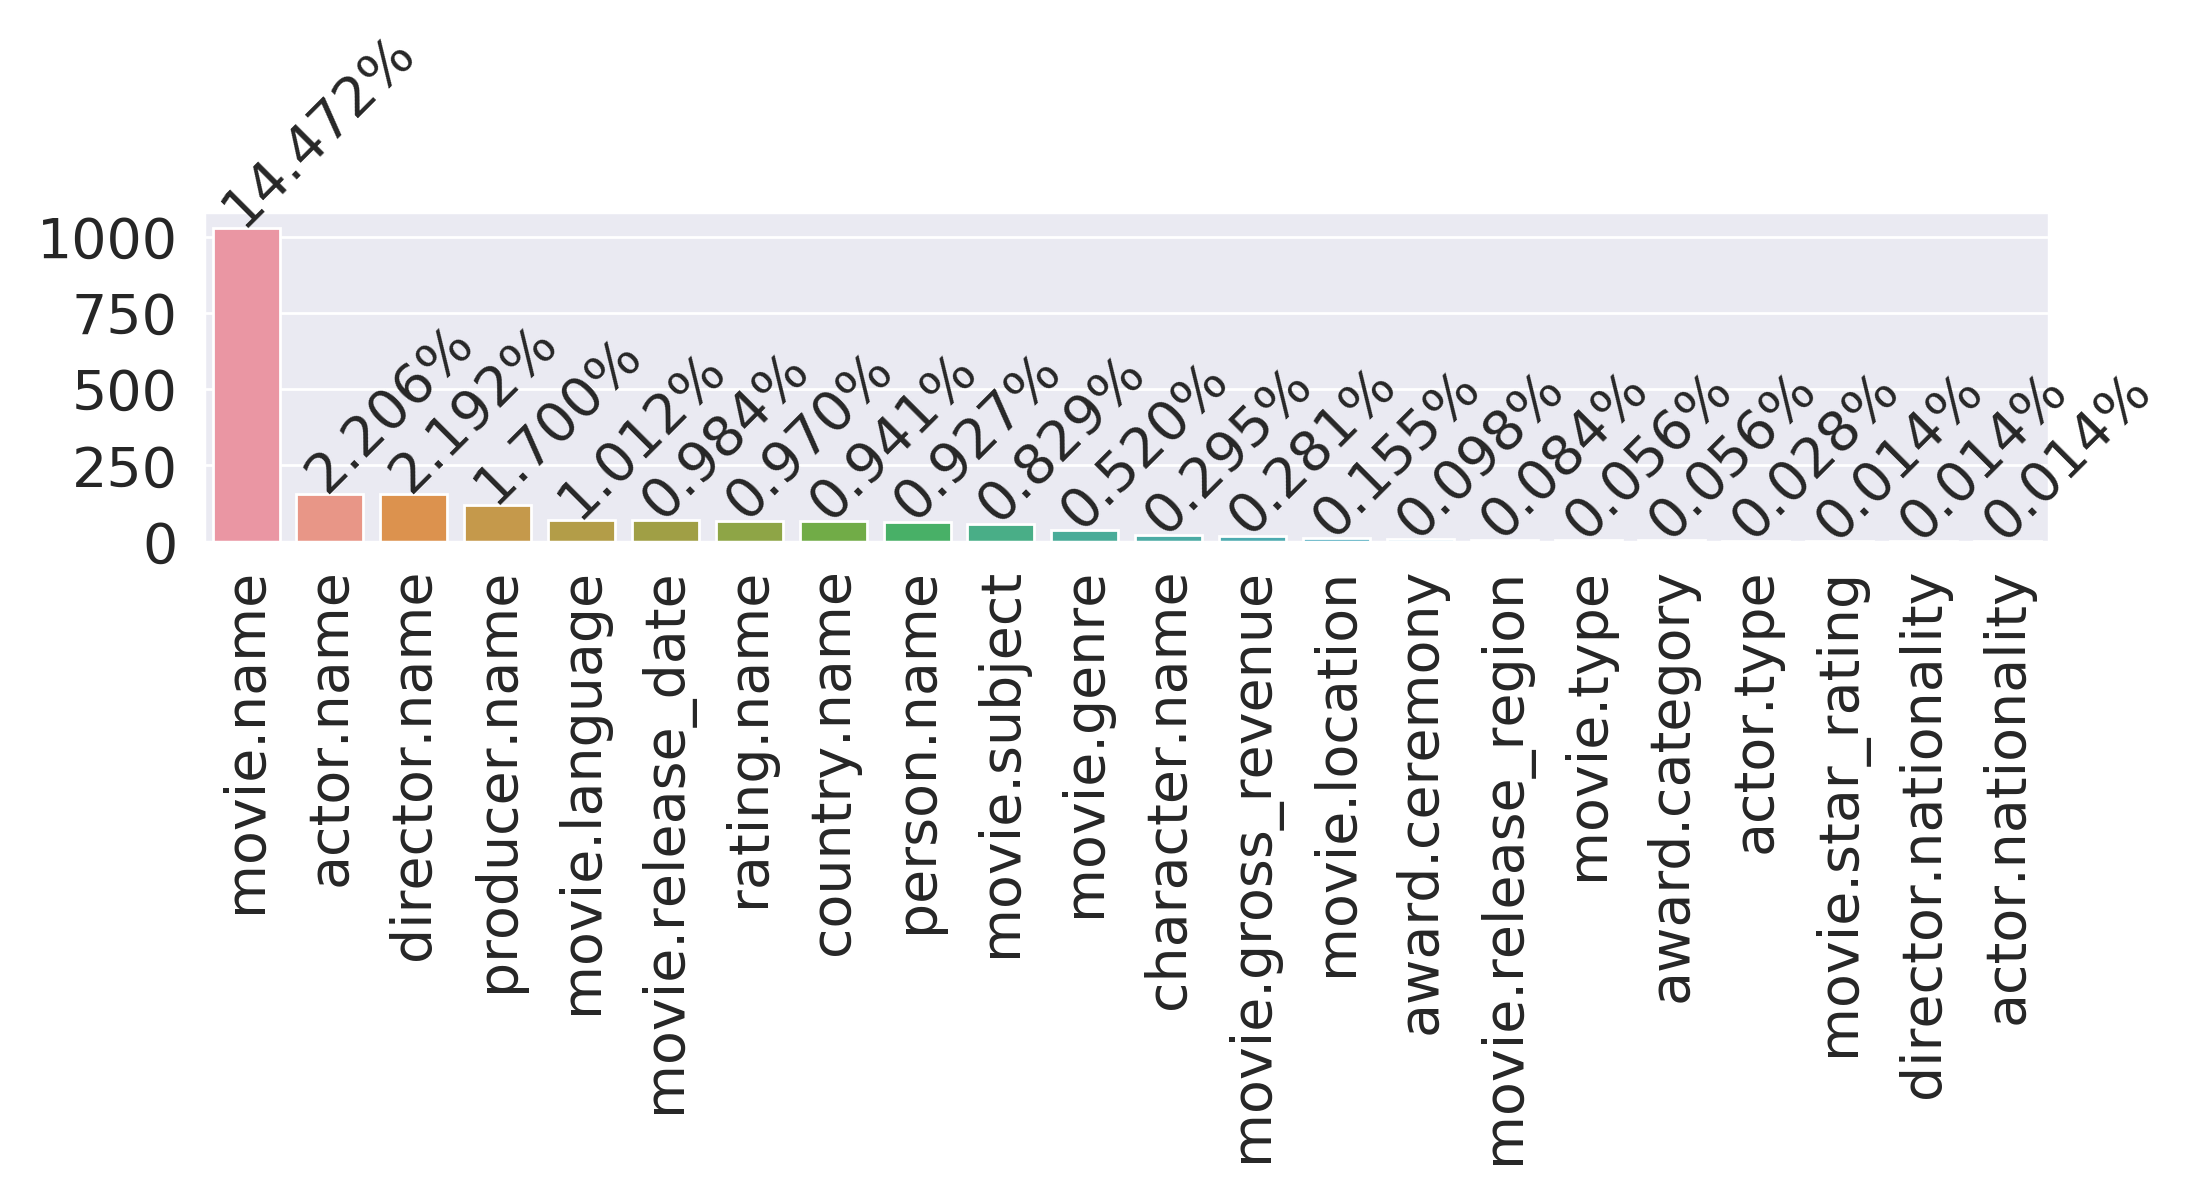
\includegraphics[width=\textwidth]{img/test-concepts-distribution}
	\caption{Test dataset.}
	\end{subfigure}
	\label{fig:concept-distribution}
	\caption{Distributions of the various concepts in the train and test datasets. The \textit{O} concept was removed to make it easier to understand the weight of the other concepts.}
\end{figure*}

\section{Results}

\section{Credits}

\end{document}
